\documentclass{report}
\usepackage{incgraph}
\usepackage{blindtext}
\usepackage[utf8]{inputenc}
\usepackage{polski}
\begin{document}

    \chapter{Przyklady zrealizowanego zakresu translacji html do latex}

    \section{Formatowanie tekstu}
        \subsection{Pogrubienie}
            \textbf{Lorem ipsum dolor sit amet, consectetur adipiscing elit.} 
            Nullam turpis erat, efficitur ac feugiat et, iaculis eget 
            risus. Cras porttitor finibus mi ut lacinia. Phasellus ut 
            ipsum semper, scelerisque justo ut, volutpat est. 

        \subsection{Kursywa}
            \textit{Phasellus euismod neque orci, non finibus lorem vestibulum nec.}

        \subsection{Podkreslenie}
            \underline{Lorem ipsum dolor sit amet, consectetur adipiscing elit.} 
            Nullam turpis erat, efficitur ac feugiat et, iaculis eget 
            risus. Cras porttitor finibus mi ut lacinia. Phasellus ut 
            ipsum semper, scelerisque justo ut, volutpat est. Donec posuere 
            tellus sed laoreet posuere. Sed eget fermentum mauris. Phasellus 
            dignissim arcu vulputate, varius dui sed, posuere leo. Morbi 
            elementum nibh at luctus cursus.
        
        \subsection{Nowa linia}
            Nullam turpis erat, efficitur ac feugiat et, iaculis eget 
            risus. Cras porttitor finibus mi ut lacinia. Phasellus ut 
            ipsum semper, scelerisque justo ut, volutpat est. \newline Donec posuere 
            tellus sed laoreet posuere. Sed eget fermentum mauris. Phasellus 
            dignissim arcu vulputate, varius dui sed, posuere leo. Morbi 
            elementum nibh at luctus cursus. 

        \subsection{Wysrodkowanie}
            \centerline{Przykladowy wysrodkowany tekst}

        \subsection{Mieszane}
            \textbf{\textit{Bolded italic}}
            \newline
            \textit{\textbf{italicBolded}}

    \section{Tabela}
        \subsection{Z obramowaniem:}
            \begin{tabular}{| c | c | c |}
                \hline
                cell7 & cell8 & cell9\\
                \hline
                cell cell & cell3 & cell3 \\
                \hline
                cell4 & cell5 & cell6 \\
                \hline
                cell4 & cell5 & cell6 \\
                \hline
                cell7 & cell8 & cell9
            \end{tabular}

        \subsection{Bez obramowania:}
            \begin{tabular}{c c c}
                cell7 & cell8 & cell9\\
                cell cell & cell3 & cell3 \\
                cell4 & cell5 & cell6 \\
                cell4 & cell5 & cell6 \\
                cell7 & cell8 & cell9  
            \end{tabular}

    \section{Wyliczenie}
        \subsection{Nieuporzadkowane}
            \begin{itemize}
                \item Wyliczenie1
                \item Wyliczenie2
                \item Wyliczenie3
            \end{itemize}

        \subsection{Uporzadkowane}
            \begin{enumerate}
                \item Wyliczenie1
                \item Wyliczenie2
                \item Wyliczenie3
            \end{enumerate}

        \subsection{Z zagniezdzeniem}
            \begin{enumerate}
                \item item1
                \item items2:
                    \textit{
                        \textbf{
                            \begin{enumerate}
                                \item item
                                \item item2 
                                \item item3 
                            \end{enumerate} 
                        }
                    }
                \item item3:
                    \begin{enumerate}
                        \item item1
                        \item item2 
                        \item item3: 
                            \begin{enumerate}
                                \item item1
                                \item item2 
                                \item item3 
                                    \begin{enumerate}
                                        \item item1
                                        \item item2 
                                        \item item3 
                                    \end{enumerate} 
                            \end{enumerate} 
                    \end{enumerate} 
            \end{enumerate}

    
    \section{Pozostale}
        \subsection{Link}
            \url{https://github.com/bartoszkordek/AGH-Jezyki-formalne-i-kompilatory}

        \subsection{Zdjecie}
            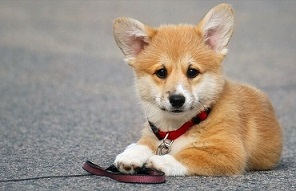
\includegraphics{corgi.jpg}

        \subsection{Przykladowa podsekcja}
            \subsubsection{Przykladowa podpodsekcja}

\end{document}